\section{Scheduling}

The control design provides task periods and profiling provides execution time specifications for
each component instance.  Data transfer rates and overhead parameters are stored
in the platform model. \cite{sched:analysis}
describes the actual constraint model details, which are an extension of earlier
work \cite{sched:offline}. The Gecode constraint programming
tool \cite{tools:gecode} solves these constraints for task release times and
message transfer times on the time-triggered platform. The scheduling process
guarantees that the implementation meets the timing requirements required by the
control design process.  The passive control design provides stability
guarantees, even in the face of timing jitter or limited message loss.  Hence
(within the bounds of acceptable delays) the scheduler does not have to account
for timing uncertainty beyond that inherent in the platform as long as the
component abstraction is preserved in all interpretations that use the
deployment information.

\begin{figure}
\centering
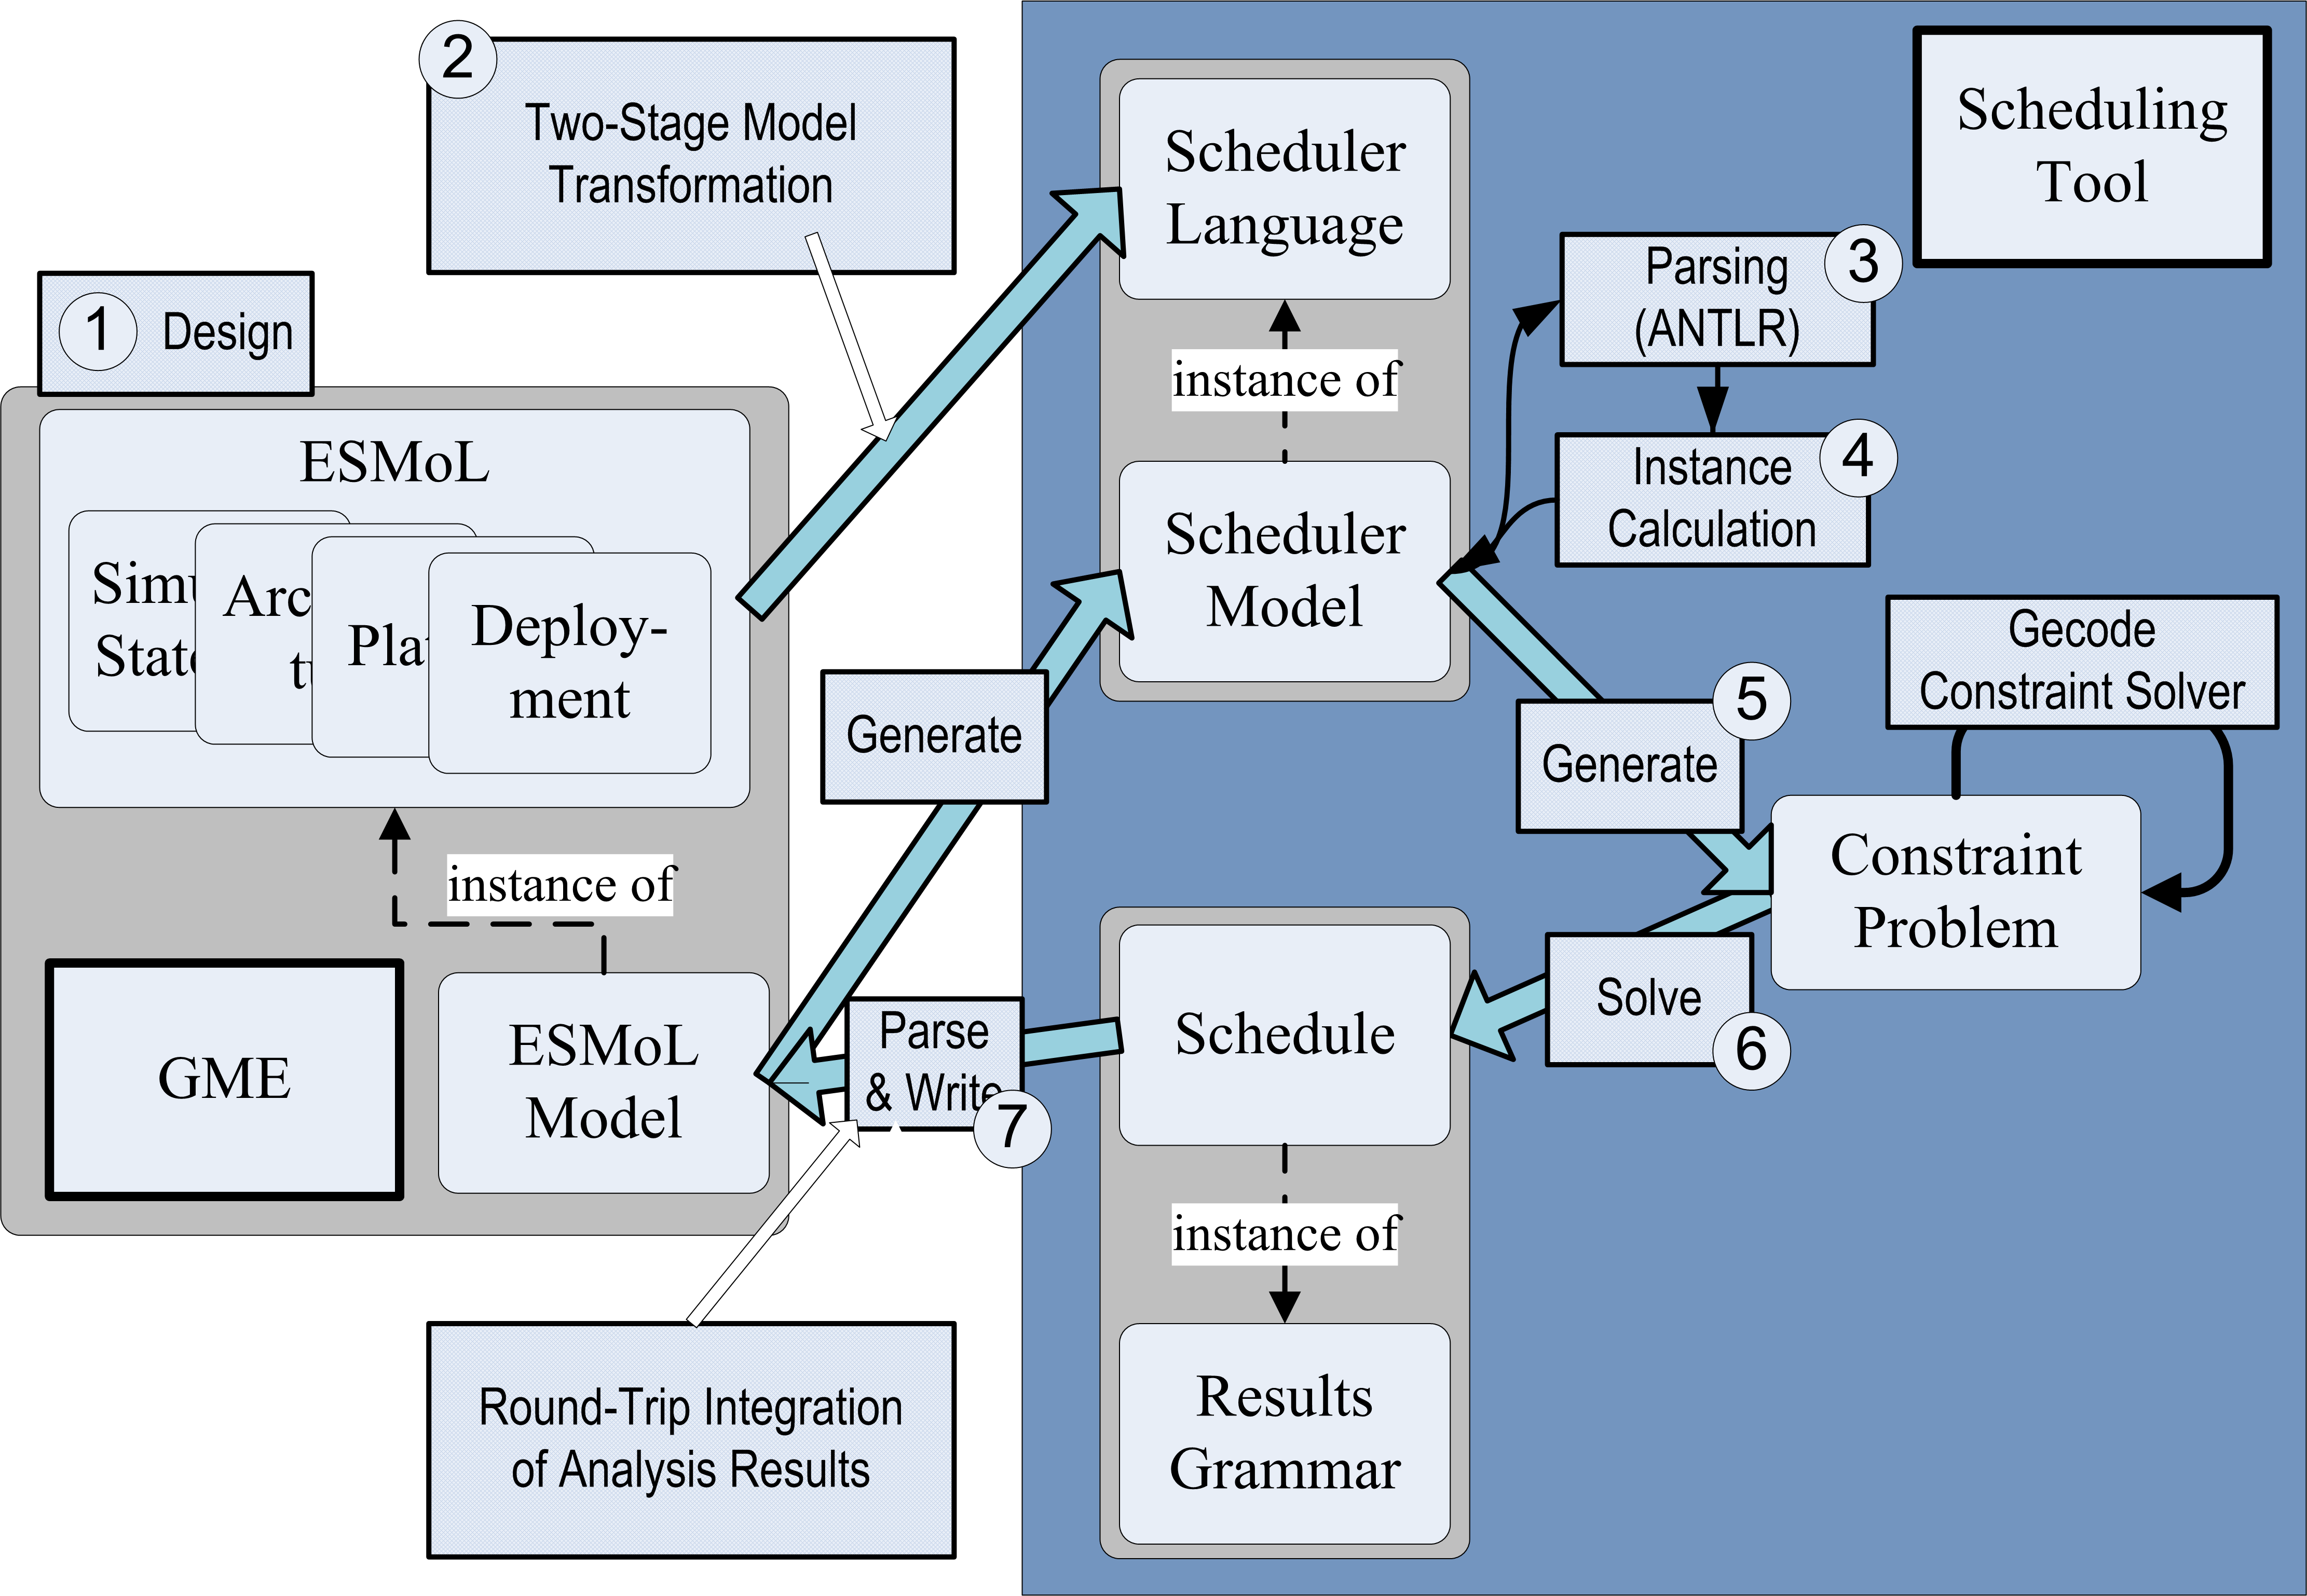
\includegraphics[width=0.85\columnwidth]{figures/sched_integration.png}
    \caption{Integration of the scheduling model by round-trip structural transformation between the language 
of the modeling tools and the analysis language.}
    \label{fig:sched_int}
\end{figure}

As the most mature analysis translator in our tools, the syntactic translation to the scheduling model 
provides the best conceptual illustration of the integration process.  Fig. \ref{fig:sched_int} shows a 
model transformation distilling details from the ESMoL tools and creating a scheduling problem model whose 
syntax represents the proper sets of behaviors.  The task and message release time results (if the schedule 
is feasible) are fed back to the modeling framework as configuration parameters.

In the example model, the configuration file created from the template is processed 
by the scheduling tool.  The resulting start times are then imported back into the
model.